\documentclass{standalone}

\usepackage{pgfplots,tikz,amsmath}
\begin{document}
    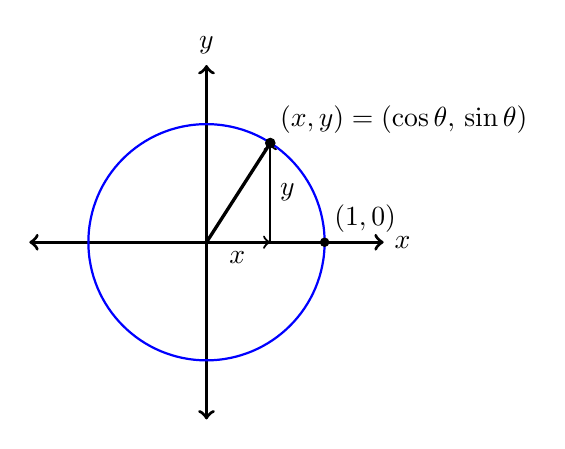
\begin{tikzpicture}[scale=1.5]
        \draw[<->, very thick] (-1.5,0) -- (1.5,0) node[anchor=west]{$x$}; 
        \draw[<->, very thick] (0,-1.5) -- (0,1.5) node[anchor=south]{$y$}; 
        \draw[thick, color=blue] (0,0) circle(1cm);
        \draw[color=black, very thick] (0,0) -- (0.54,0.84);
        \draw[color=black,fill=black] (0.54,0.84) circle(0.04cm)
        node[anchor=south west]{$(x,y)=(\cos\theta,\,\sin\theta)$};
        \draw[->, thick] (0,0) -- (0.54,0);
        \draw[->, thick] (0.54,0) -- (0.54,0.84);
        \draw (0.26,0) node[anchor=north]{$x$};
        \draw (0.54,0.42) node[anchor=west]{$y$};
        \draw[color=black, fill=black] (1,0) circle(0.035cm) node[anchor=south
        west]{$(1,0)$};
    \end{tikzpicture}
\end{document}
